%!TEX root = ../preamble.tex






\definecolor{cpurple}{HTML}{BA6FB6}
\definecolor{corange}{HTML}{FDAE61}
\definecolor{cgreen}{HTML}{ABDDA4}
\definecolor{cblue}{HTML}{2B83BA}

\begin{figure}[H]
\centering
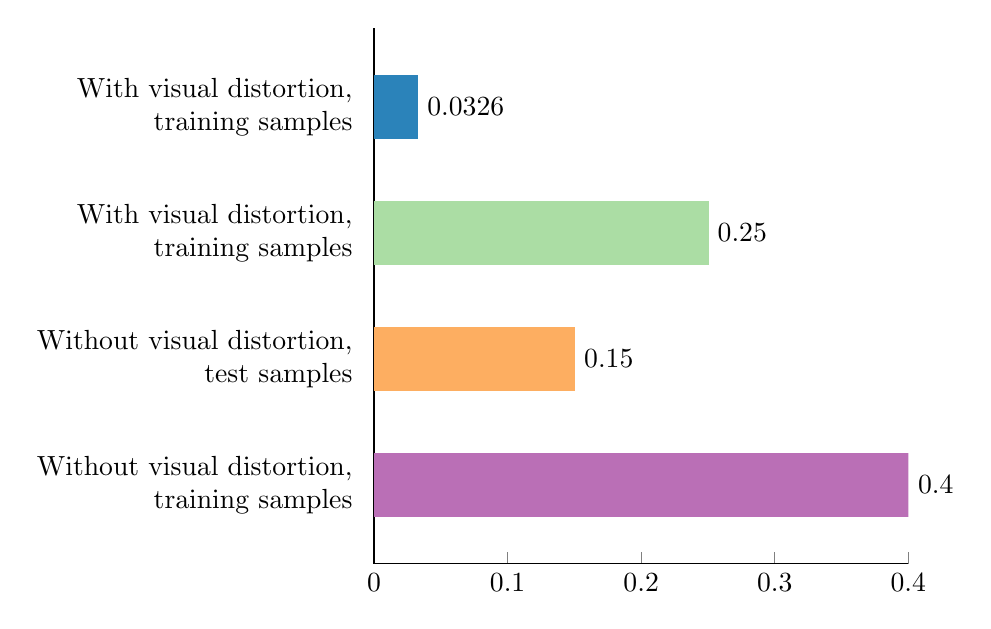
\begin{tikzpicture}
\begin{axis}[
    xbar=0pt,
    /pgf/bar shift=0pt,
    legend style={
    legend columns=4,
        at={(xticklabel cs:0.5)},
        anchor=north,
        draw=none
    },
    ytick={0,...,3},
    ytick style={draw=none},
    axis y line*=none,
    axis x line*=bottom,
    xtick={0,0.1,...,0.5},
    width=.69\textwidth,
    bar width=8mm,
	yticklabels={	{Without visual distortion,\\training samples}, 
						{Without visual distortion,\\test samples}, 
						{With visual distortion,\\training samples}, 
						{With visual distortion,\\training samples}, 
	},
	yticklabel style={align=right},
    xmin=0,
    xmax=0.4,
    area legend,
    y=16mm,
    enlarge y limits={abs=0.625},
    nodes near coords,
    every node near coord/.style={/pgf/number format/fixed, /pgf/number format/precision=5, text=black},
    every axis plot/.append style={fill}
]
\addplot[cpurple] coordinates {(0.400,0)};
\addplot[corange] coordinates {(0.150,1)};
\addplot[cgreen] coordinates {(0.250,2)};
\addplot[cblue] coordinates {(0.0326,3)};
\end{axis}  
\end{tikzpicture}
\caption{X}
\label{fig:stats}
\end{figure}

















































